\documentclass[../main.tex]{subfiles}

\begin{document}
\section{Results}
The results section presents the findings from the analysis of the accelerometer data collected during the simulated intrusion attempts on the MediColbox. The accelerometer data provides insights into the physical movements and vibrations experienced by the MediColbox during these intrusion scenarios.

\subsection{Analysis of Accelerometer Data}

The accelerometer data captured the accelerative patterns resulting from different simulated intrusion attempts, including striking, dropping, sawing, and shaking the MediColbox. The data analysis focused specifically on the accelerometer readings to evaluate the sensitivity and effectiveness of the IMU in detecting unauthorized access.

\clearpage

\subsubsection{Striking the MediColbox}

Figure \ref{fig:accelerometer_striking} presents the
accelerometer data recorded when the MediColbox was
struck with a fist.
The accelerometer readings showed a sharp increase in
acceleration followed by a swift, but gradual decrease as
the impact dissipated.
The peak acceleration value reached during the
strike was measured at
$X = 5 [m/s^2]$, $Y = -31 [m/s^2]$, $Z = -55 [m/s^2]$
and occurred at $t = 0.8[s]$.
The analysis of the data indicates that the
IMU successfully detected and recorded the impact caused by the
striking event.

\begin{figure}[htbp]
\centering
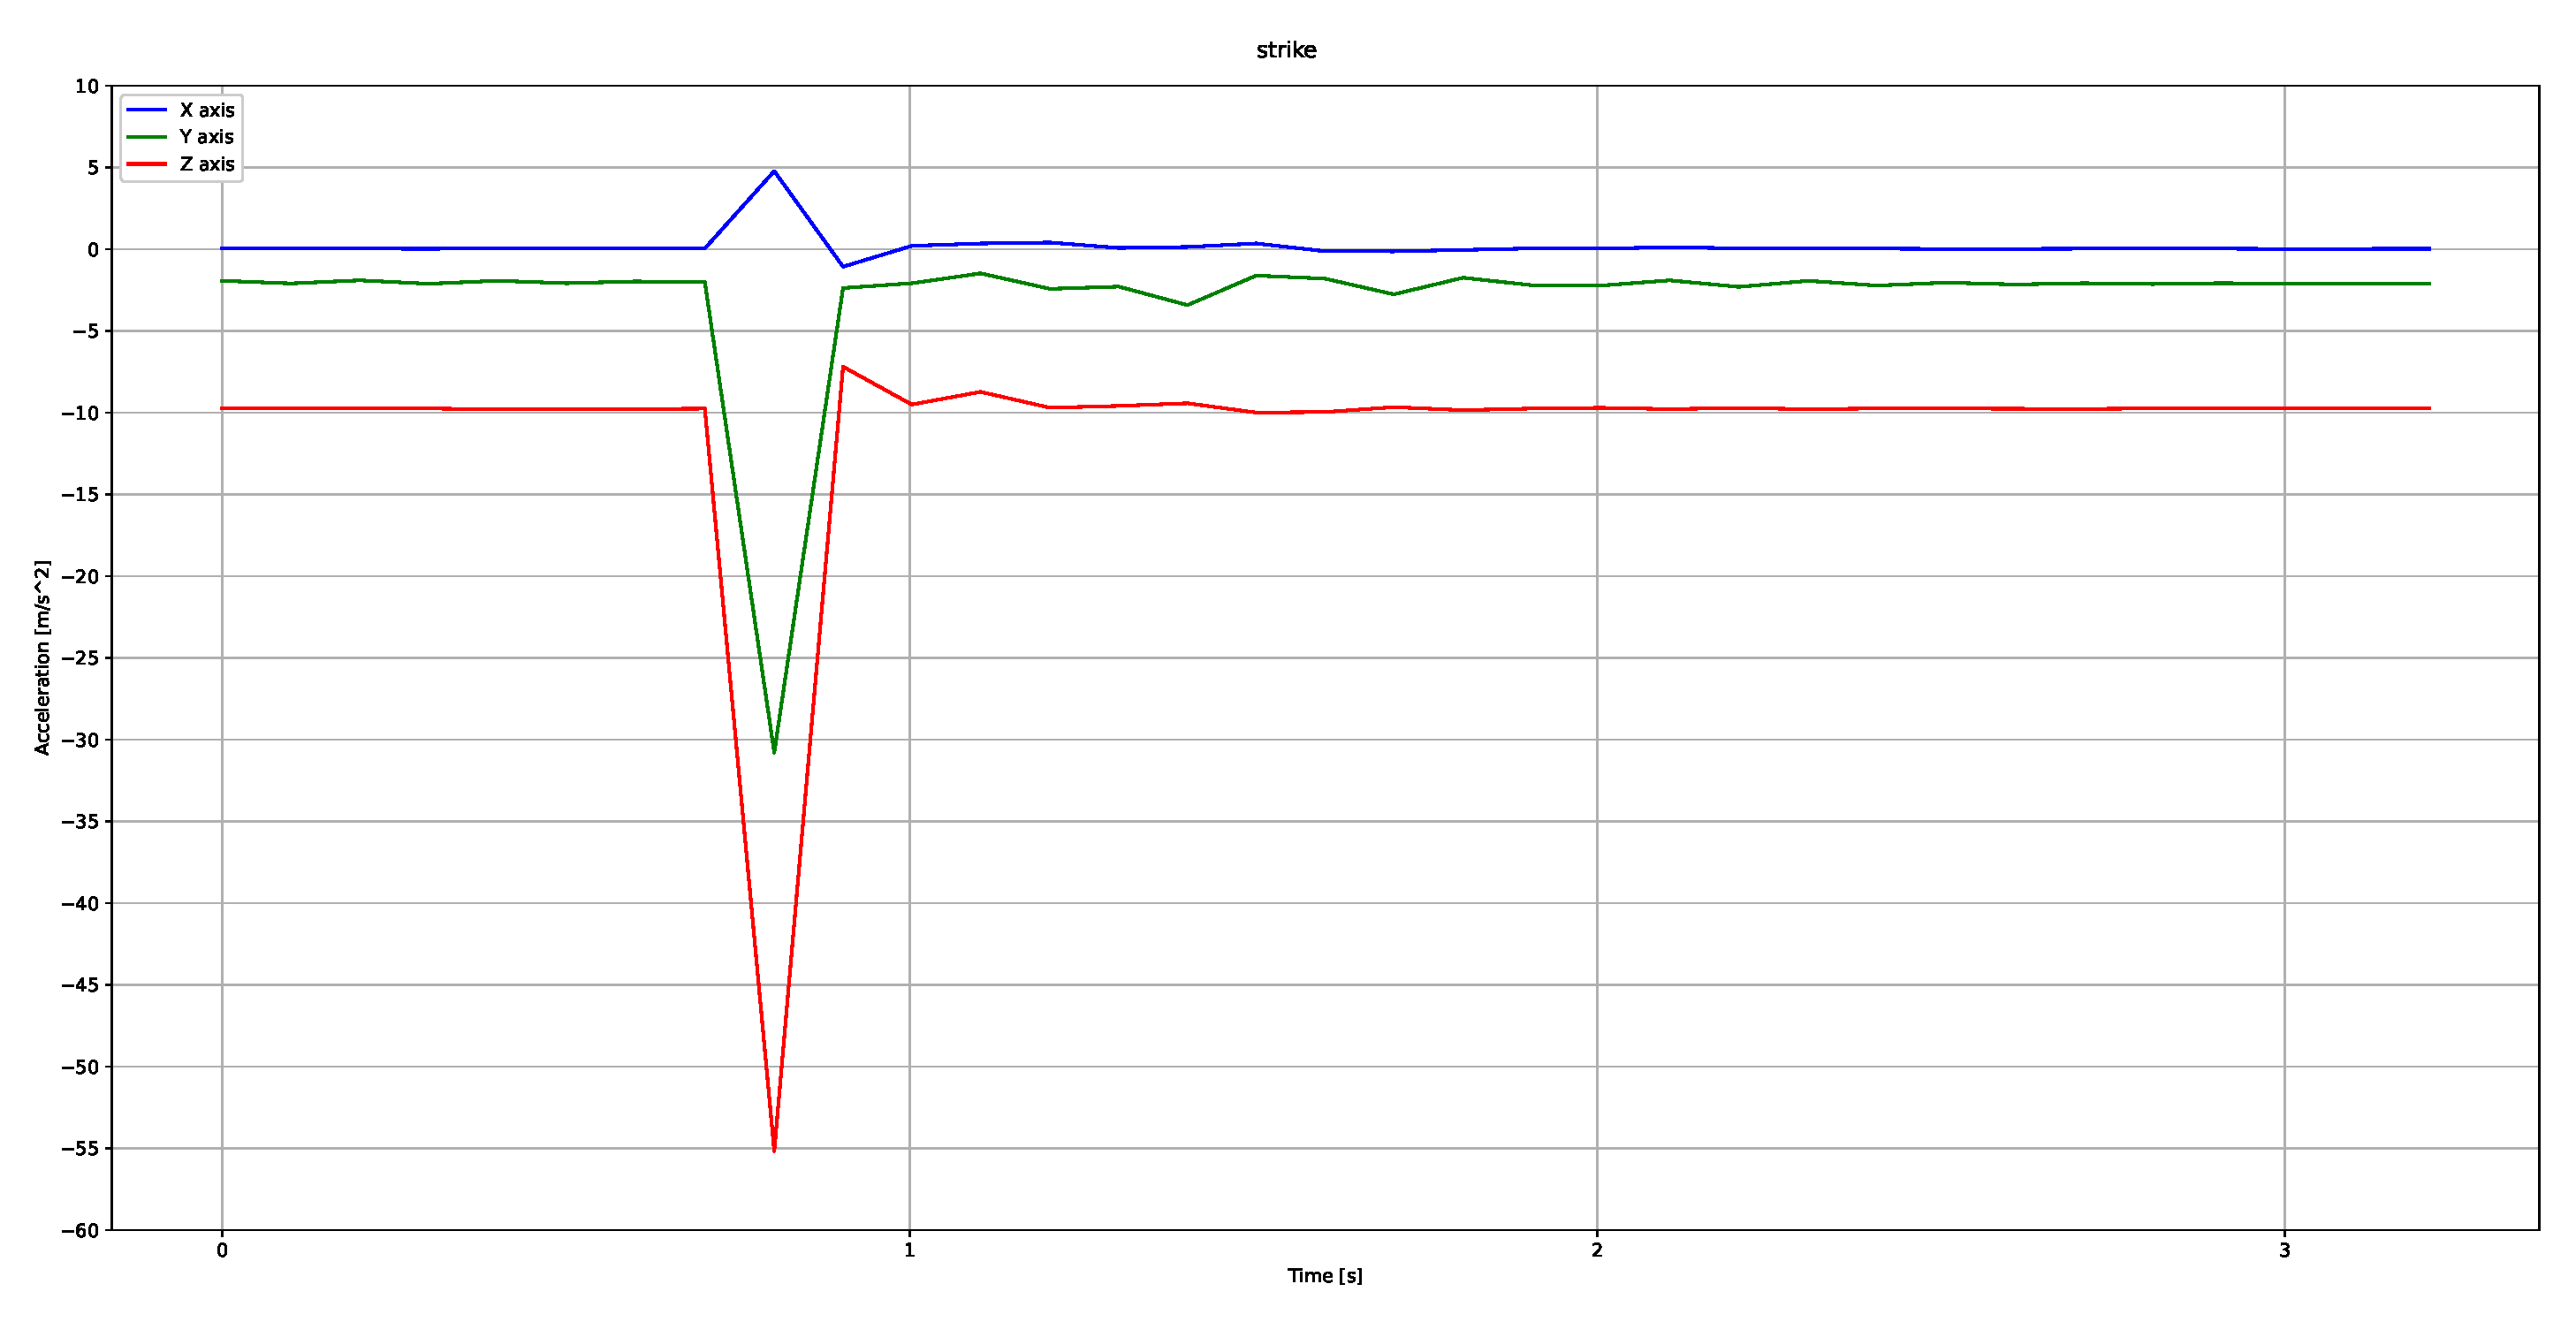
\includegraphics[width=0.8\textwidth]{resources/figures/Acceleration_strike.eps}
\caption{Accelerometer data during the striking event}
\label{fig:accelerometer_striking}
\end{figure}

The Fourier analysis of the accelerometer data during the
striking event is shown in
Figure \ref{fig:fourier_accelerometer_striking}.
The Fourier analysis allows us to examine the
frequency components present in the accelerometer readings and
provides insights into the characteristics of the
impact and resulting vibrations.
By analyzing the frequency distribution and
identifying prominent peaks or patterns in the frequency domain,
we can gain a deeper understanding of the
dynamic response of the MediColbox to external forces.

\begin{figure}[htbp]
\centering
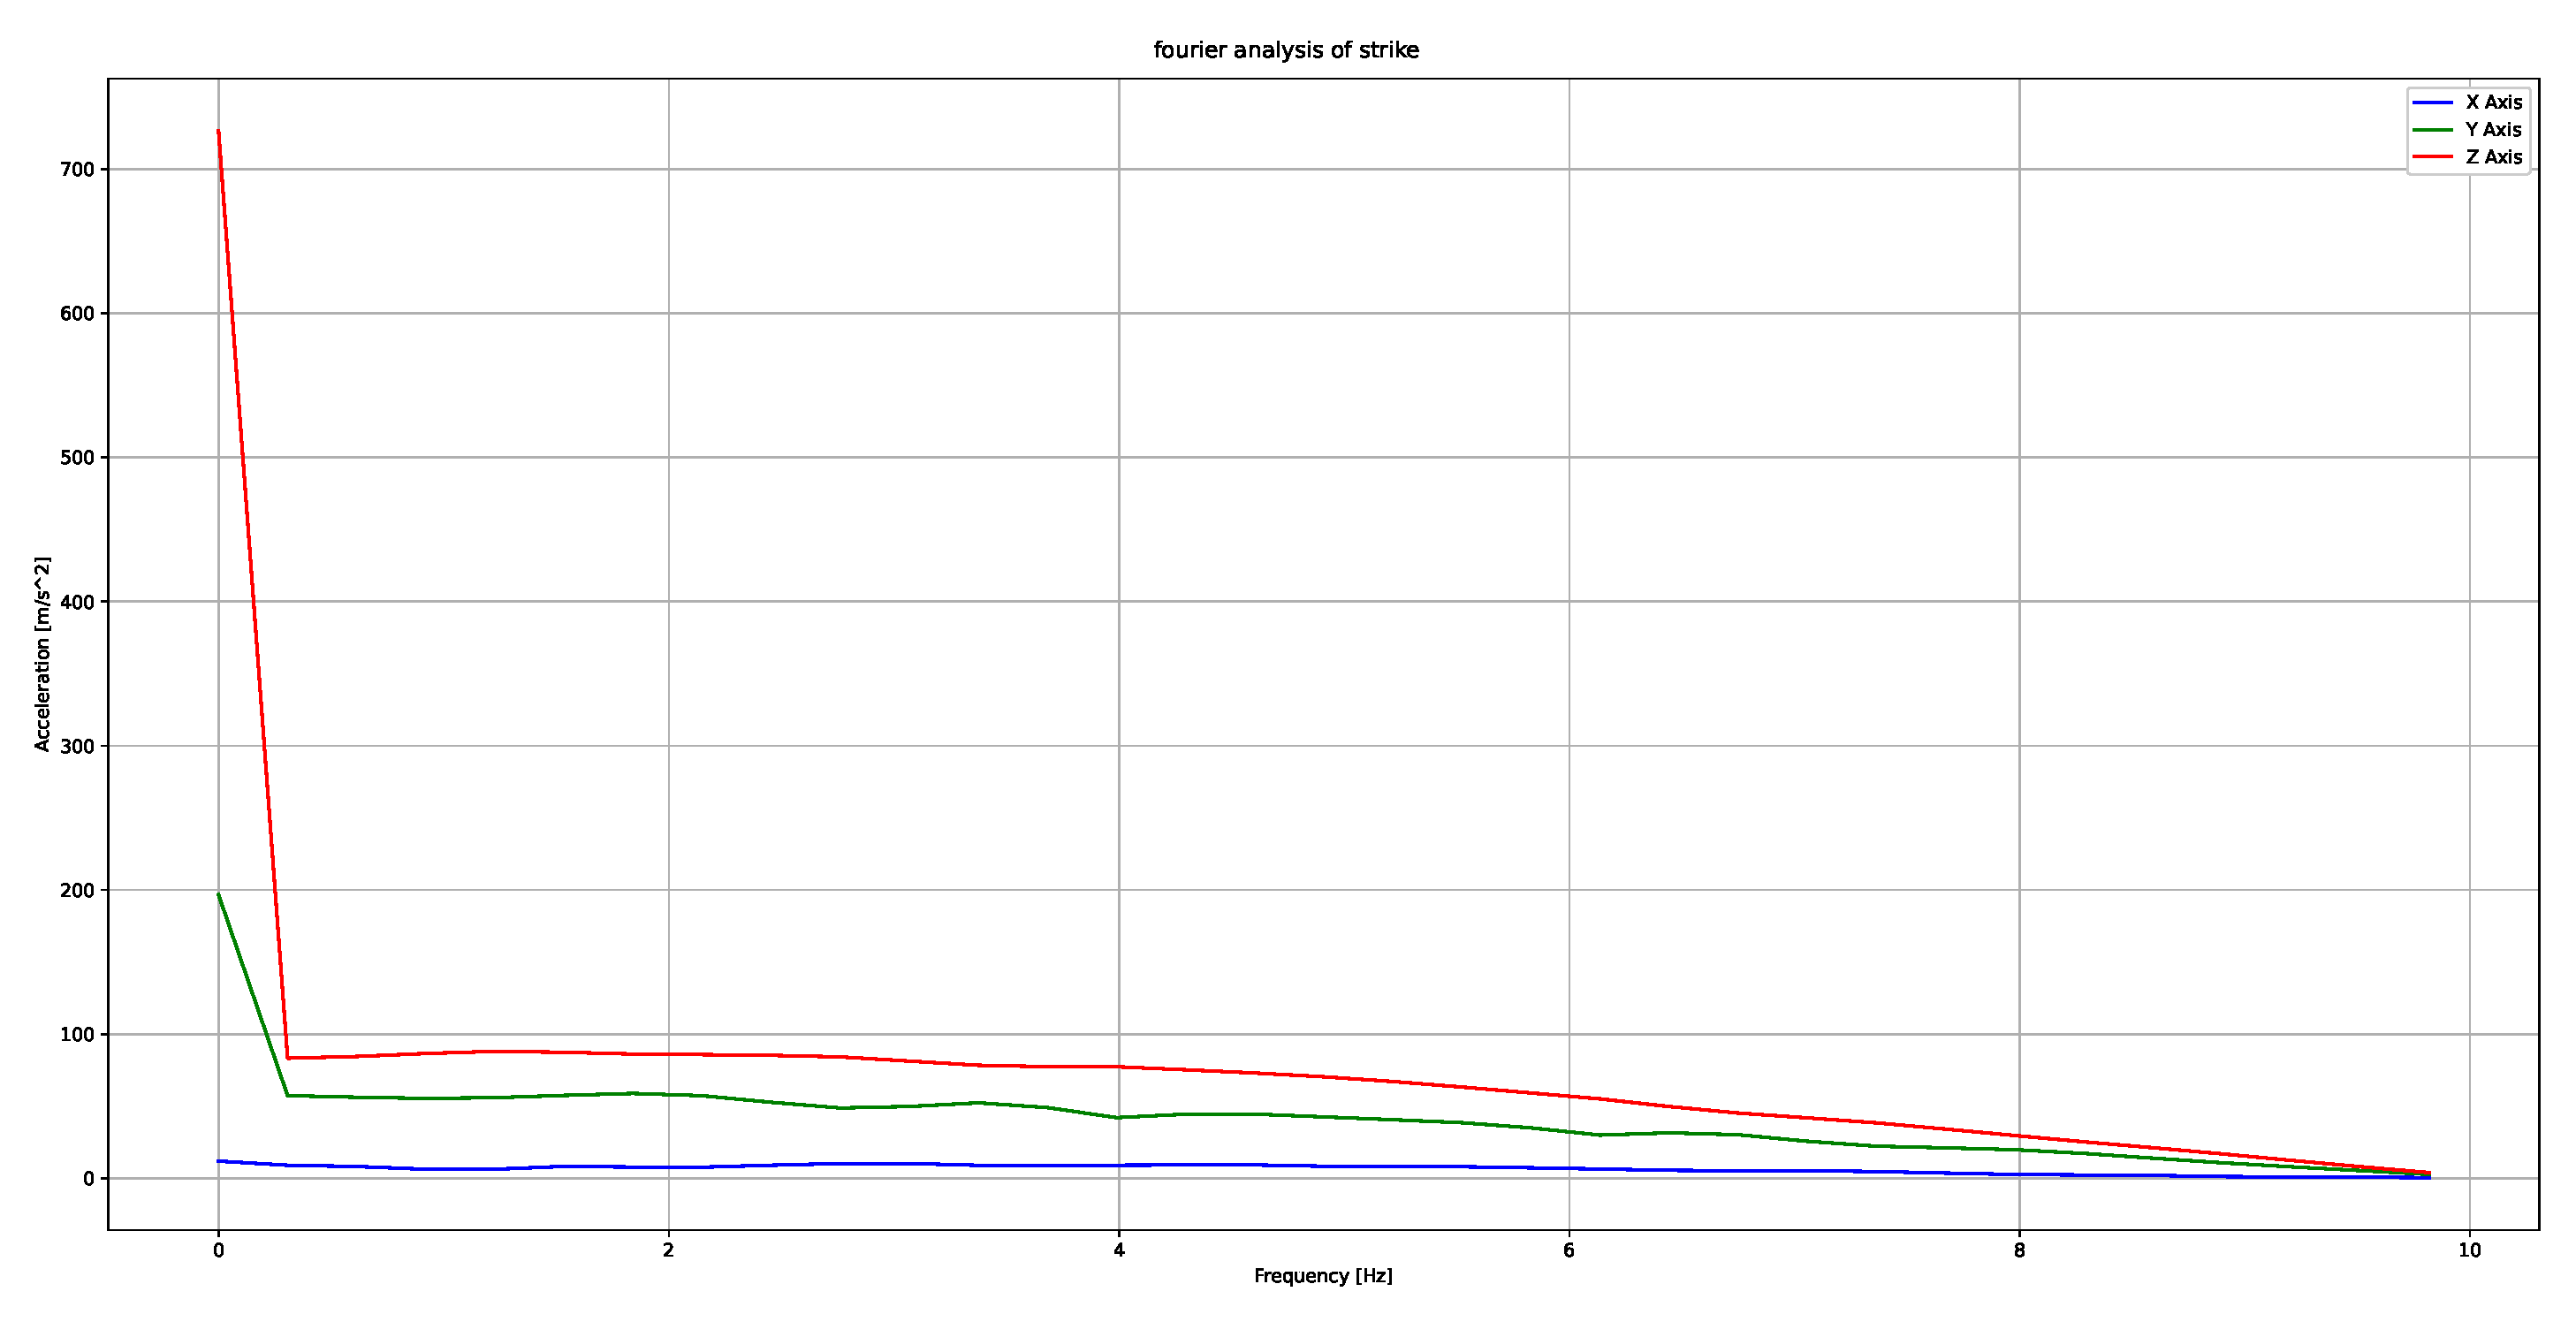
\includegraphics[width=0.8\textwidth]{resources/figures/Fourier_acceleration_strike.eps}
\caption{Fourier analysis of accelerometer data during the striking event}
\label{fig:fourier_accelerometer_striking}
\end{figure}

\clearpage
\subsubsection{Dropping the MediColbox}

The accelerometer data collected when the MediColbox was
dropped from a table is presented in
Figure \ref{fig:accelerometer_dropping}.
The data showed a sudden increase in acceleration when the
MediColbox was released,
followed by a deceleration as it came into contact with the
surface. The maximum acceleration value recorded during the
drop was
$X = -7.7 [m/s^2]$, $Y = 35 [m/s^2]$, $Z = -50.7 [m/s^2]$,
which occurred at $t = 5.1[s]$.
The analysis confirms that the IMU effectively captured the
acceleration changes associated with the dropping event.

\begin{figure}[htbp]
    \centering
    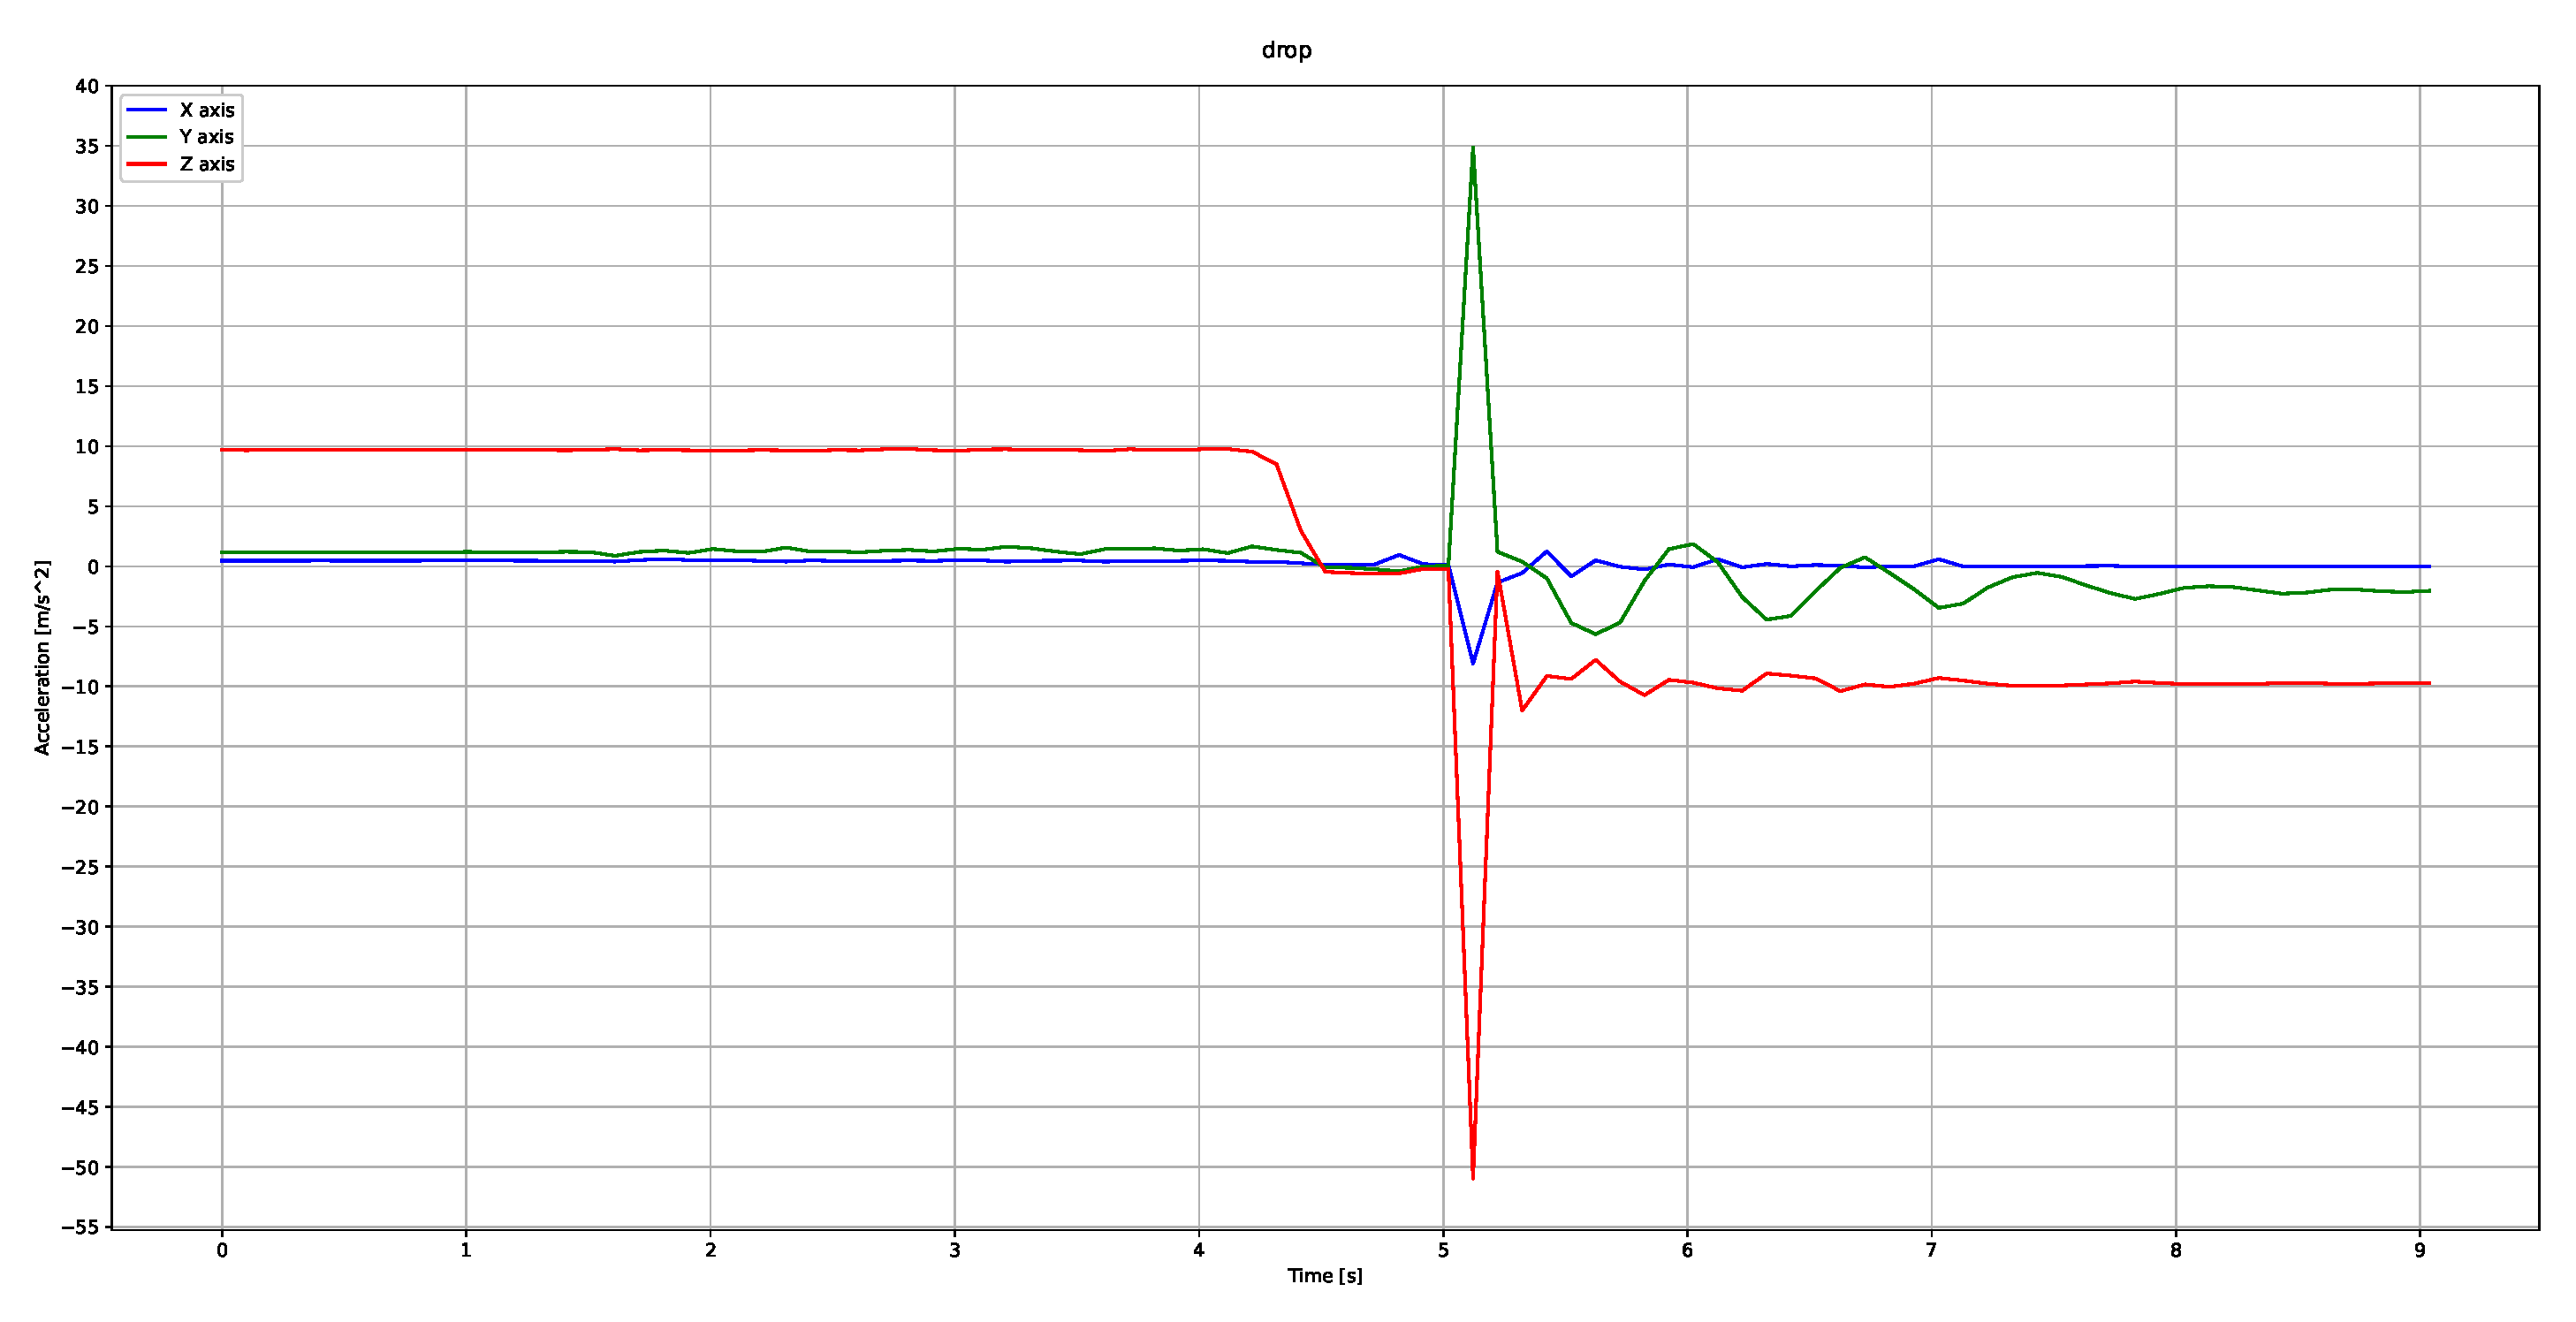
\includegraphics[width=0.8\textwidth]{resources/figures/Acceleration_drop.eps}
    \caption{Accelerometer data during the dropping event}
    \label{fig:accelerometer_dropping}
\end{figure}

The Fourier analysis of the accelerometer data during the
dropping event is shown in
Figure \ref{fig:fourier_accelerometer_dropping}.
The Fourier analysis allows us to examine the
frequency components present in the accelerometer readings and
provides insights into the characteristics of the
drop and resulting vibrations.

\begin{figure}[htbp]
    \centering
    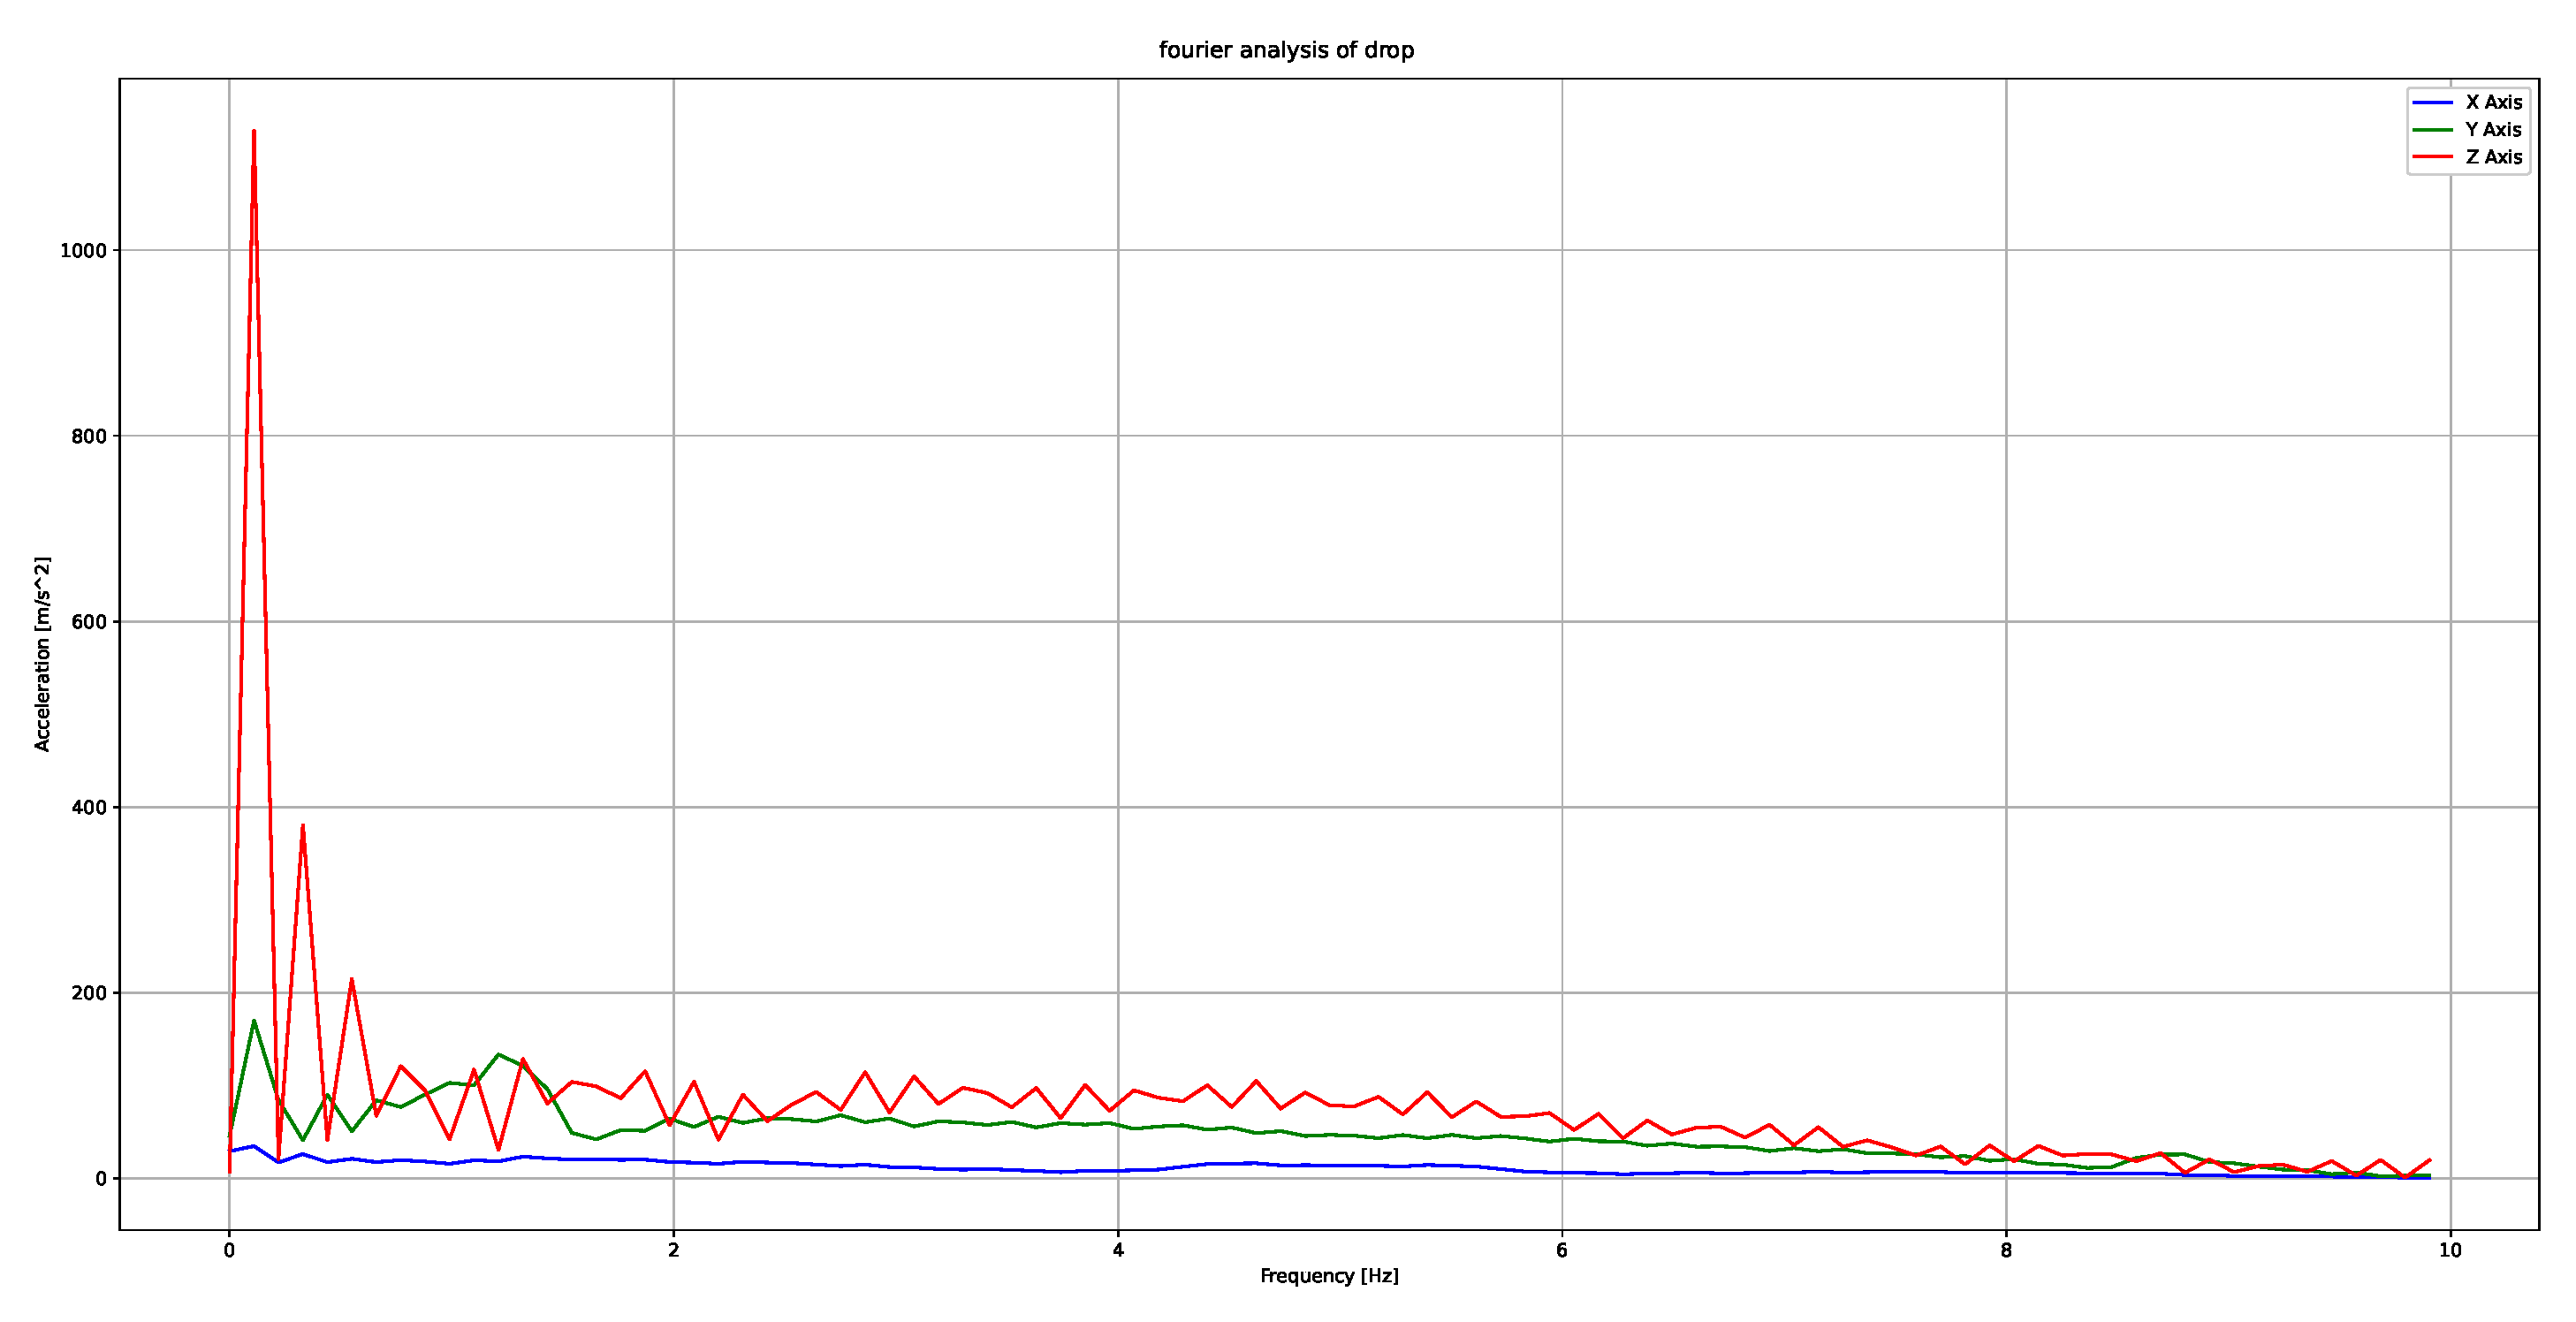
\includegraphics[width=0.8\textwidth]{resources/figures/Fourier_acceleration_drop.eps}
    \caption{Fourier analysis of accelerometer data during the dropping event}
    \label{fig:fourier_accelerometer_dropping}
\end{figure}

\clearpage

\subsubsection{Sawing on the MediColbox}

Figure \ref{fig:accelerometer_sawing} illustrates the
accelerometer data recorded while sawing on the
MediColbox using a metal cutting saw.
The data exhibited periodic variations in acceleration
corresponding to the back-and-forth sawing motion.
The analysis of the data indicated a consistent pattern of
acceleration changes during the sawing event. This suggests that the IMU was able to capture the vibrations and oscillations caused by the sawing action.

\begin{figure}[htbp]
    \centering
    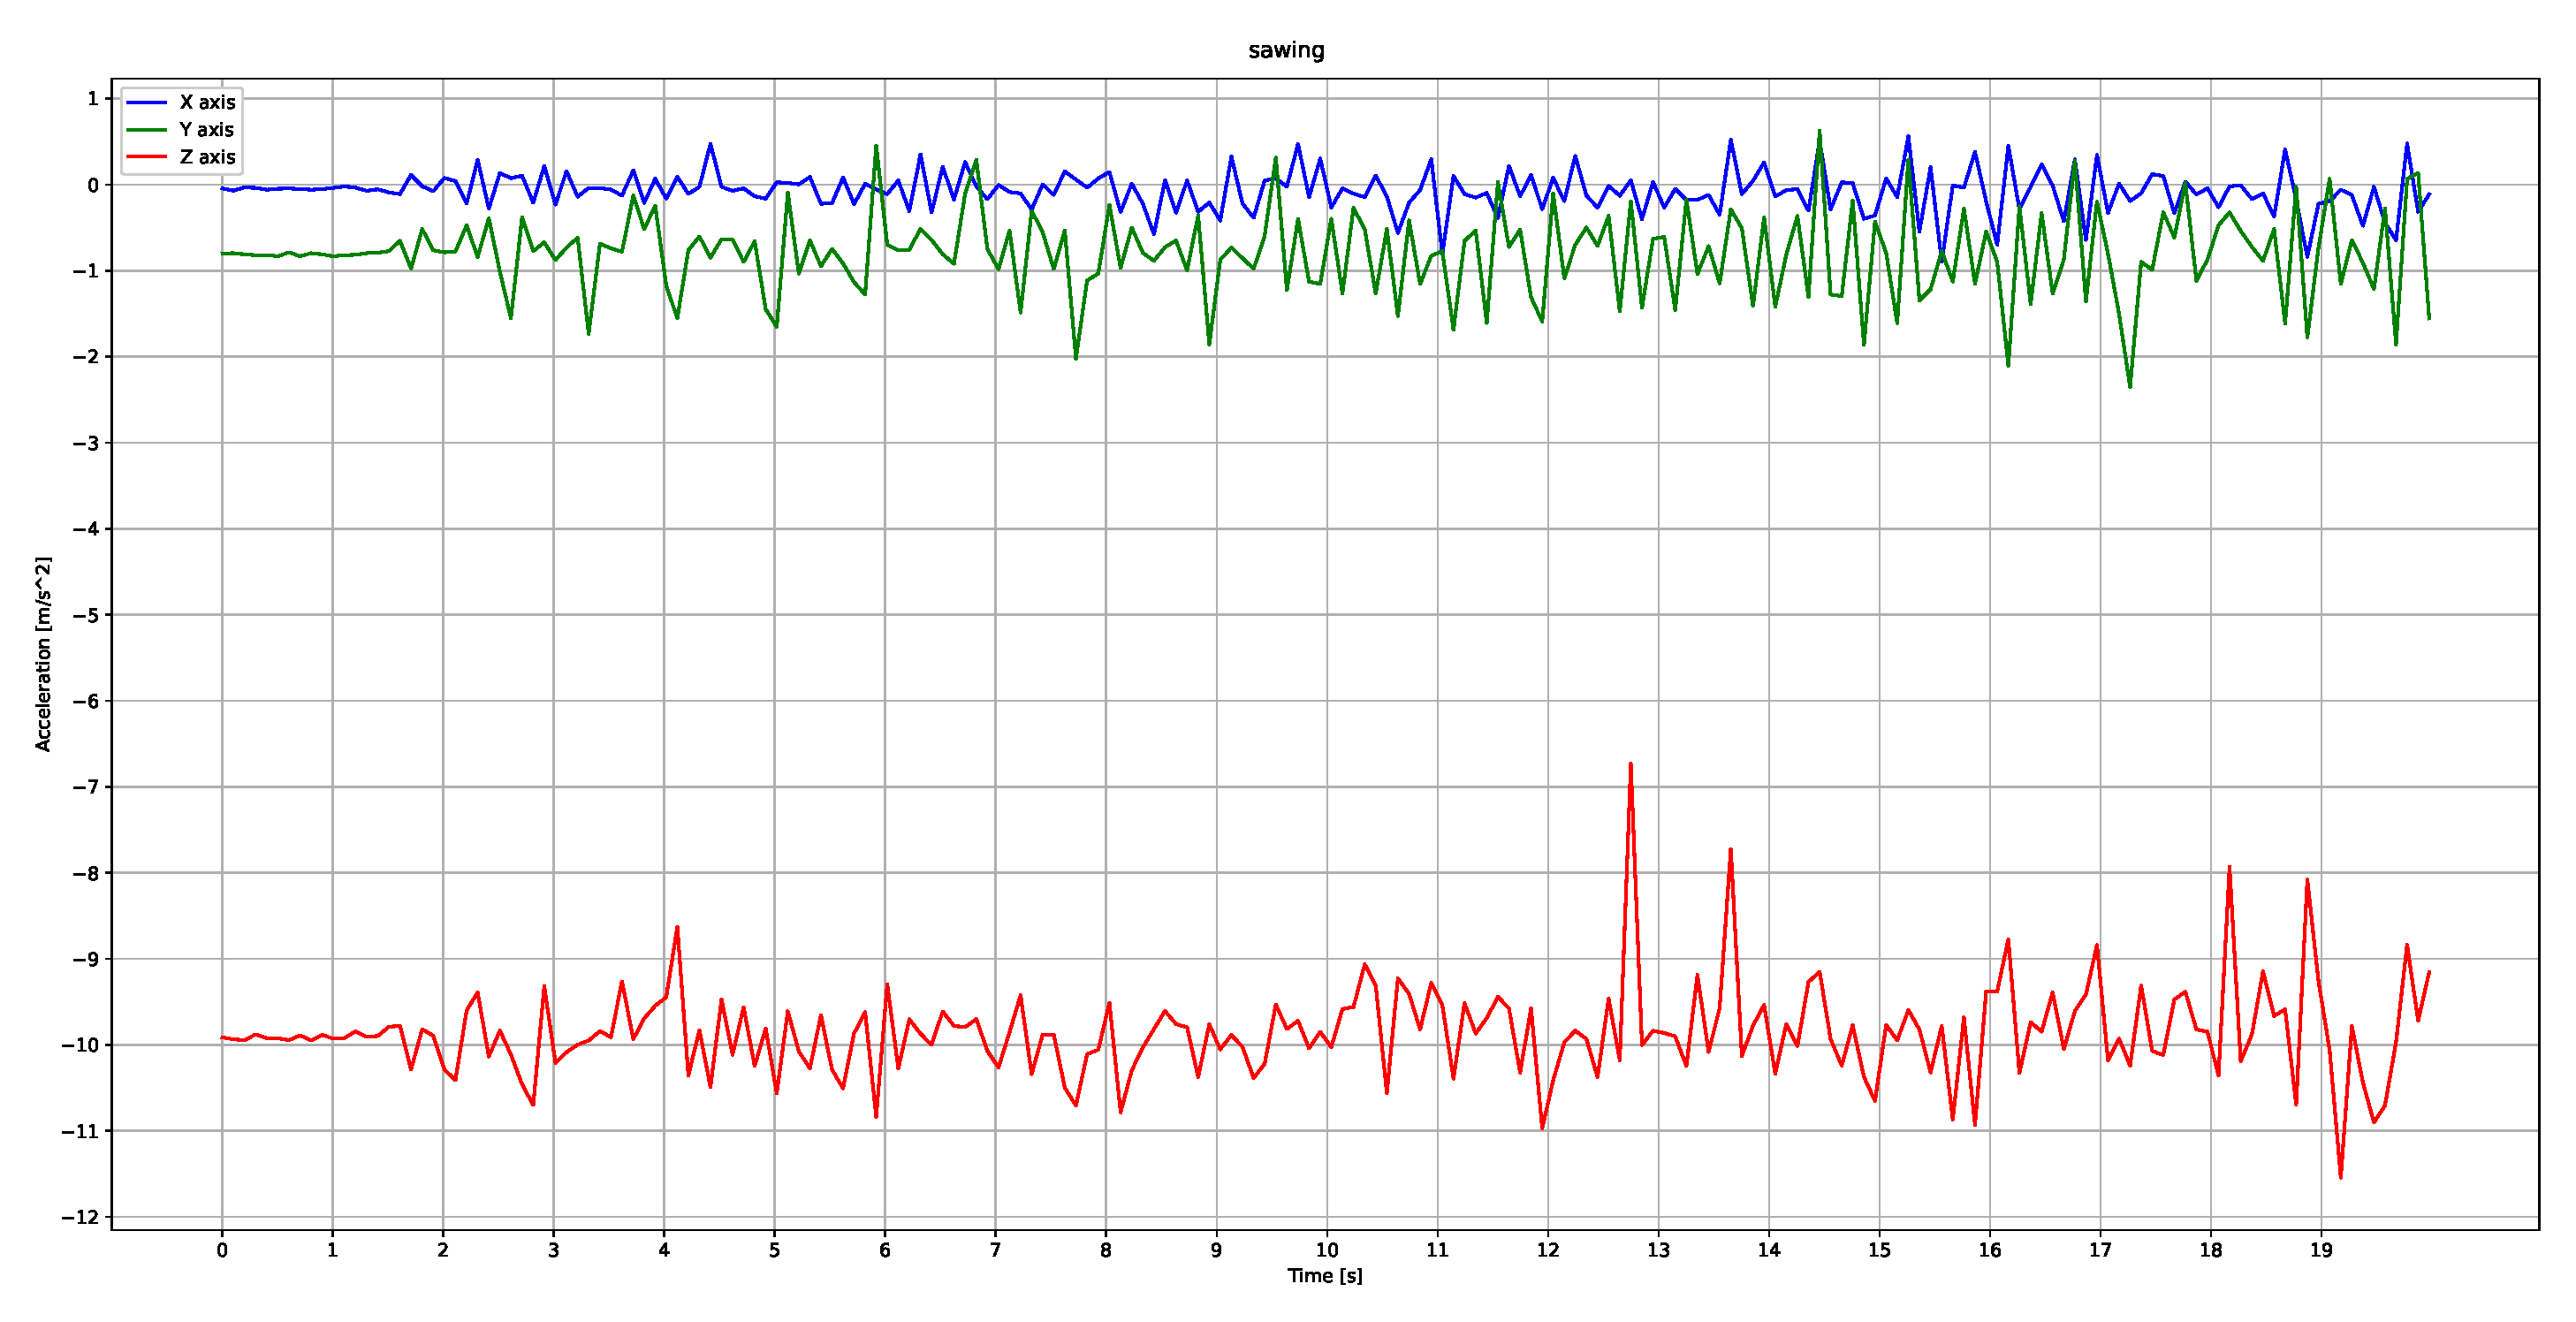
\includegraphics[width=0.8\textwidth]{resources/figures/Acceleration_sawing.eps}
    \caption{Accelerometer data during the sawing event}
    \label{fig:accelerometer_sawing}
\end{figure}

The Fourier analysis of the accelerometer data during the sawing event is shown in Figure \ref{fig:fourier_accelerometer_sawing}. The Fourier analysis allows us to examine the frequency components present in the accelerometer readings and provides insights into the characteristics of the sawing action. By analyzing the frequency distribution and identifying prominent peaks or patterns in the frequency domain, we can gain a deeper understanding of the dynamic response of the MediColbox to the sawing forces.

\begin{figure}[htbp]
    \centering
    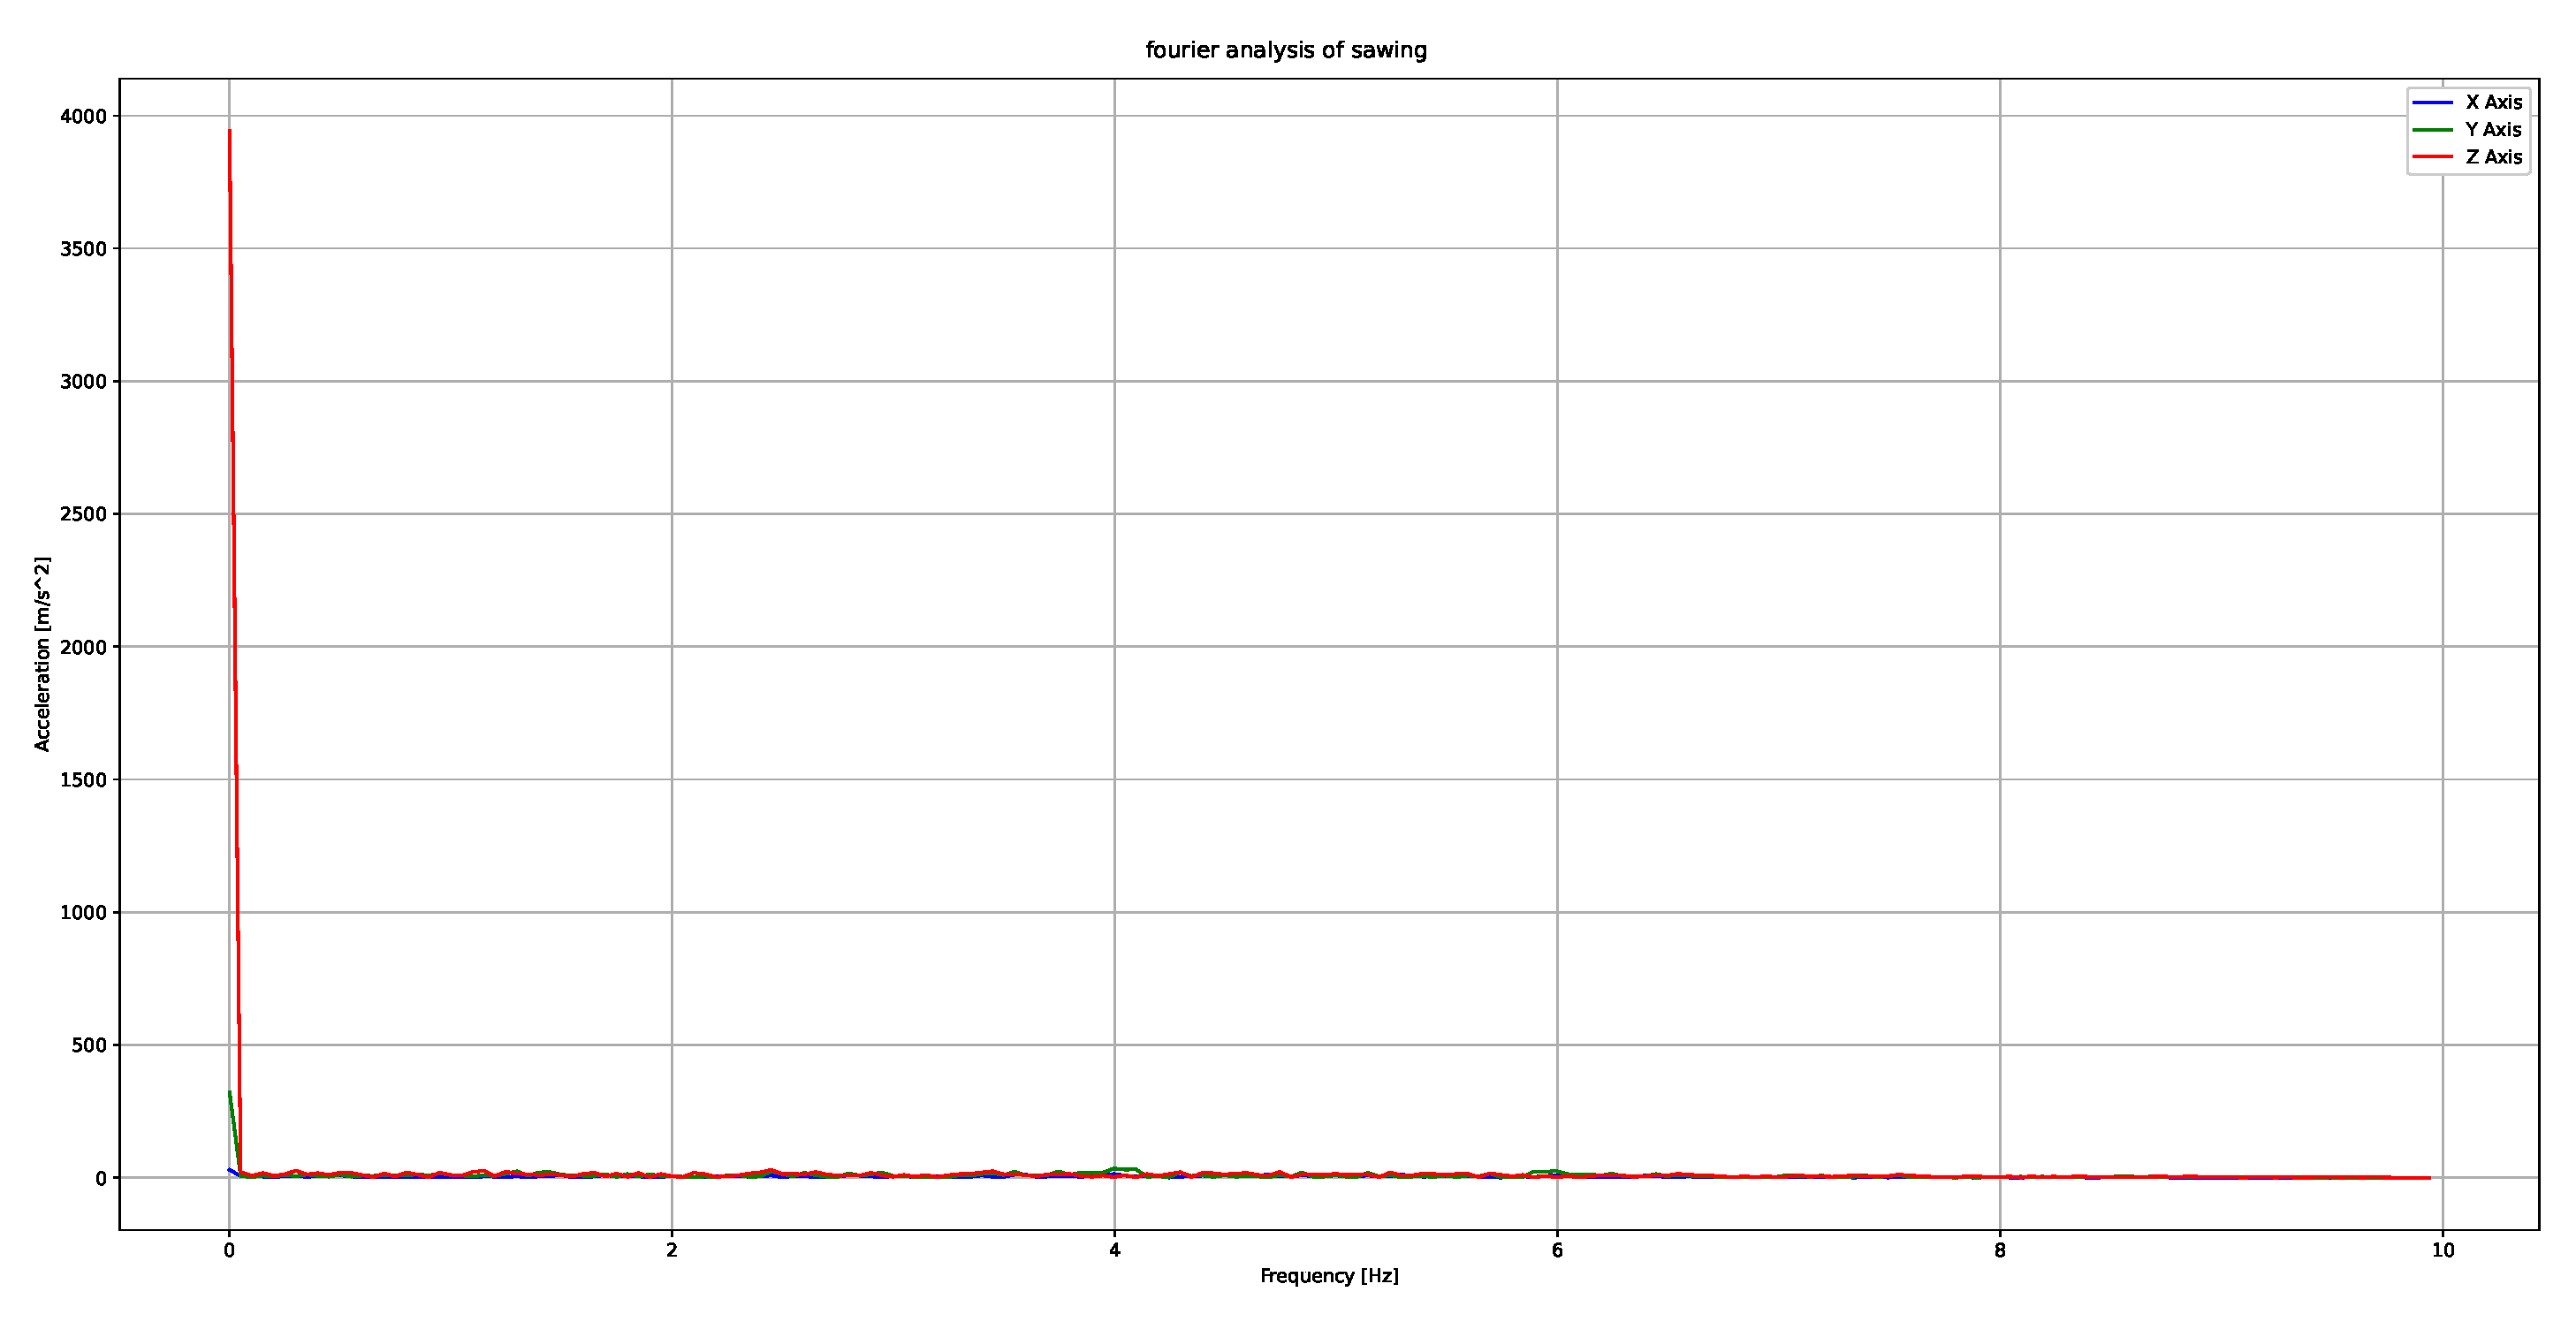
\includegraphics[width=0.8\textwidth]{resources/figures/Fourier_acceleration_sawing.eps}
    \caption{Fourier analysis of accelerometer data during the sawing event}
    \label{fig:fourier_accelerometer_sawing}
\end{figure}

\clearpage

\subsubsection{Shaking the MediColbox}

The accelerometer data obtained while shaking the
MediColbox on a sifter,
simulating cutting it with an angle grinder,
is presented in Figure \ref{fig:accelerometer_shaking}.
The data exhibited irregular and rapid fluctuations in
acceleration due to the shaking motion.
The analysis of the data demonstrated that the IMU was
sensitive enough to detect and record these rapid changes in
acceleration, indicating its potential for
detecting unauthorized access attempts involving
similar movements.

\begin{figure}[htbp]
    \centering
    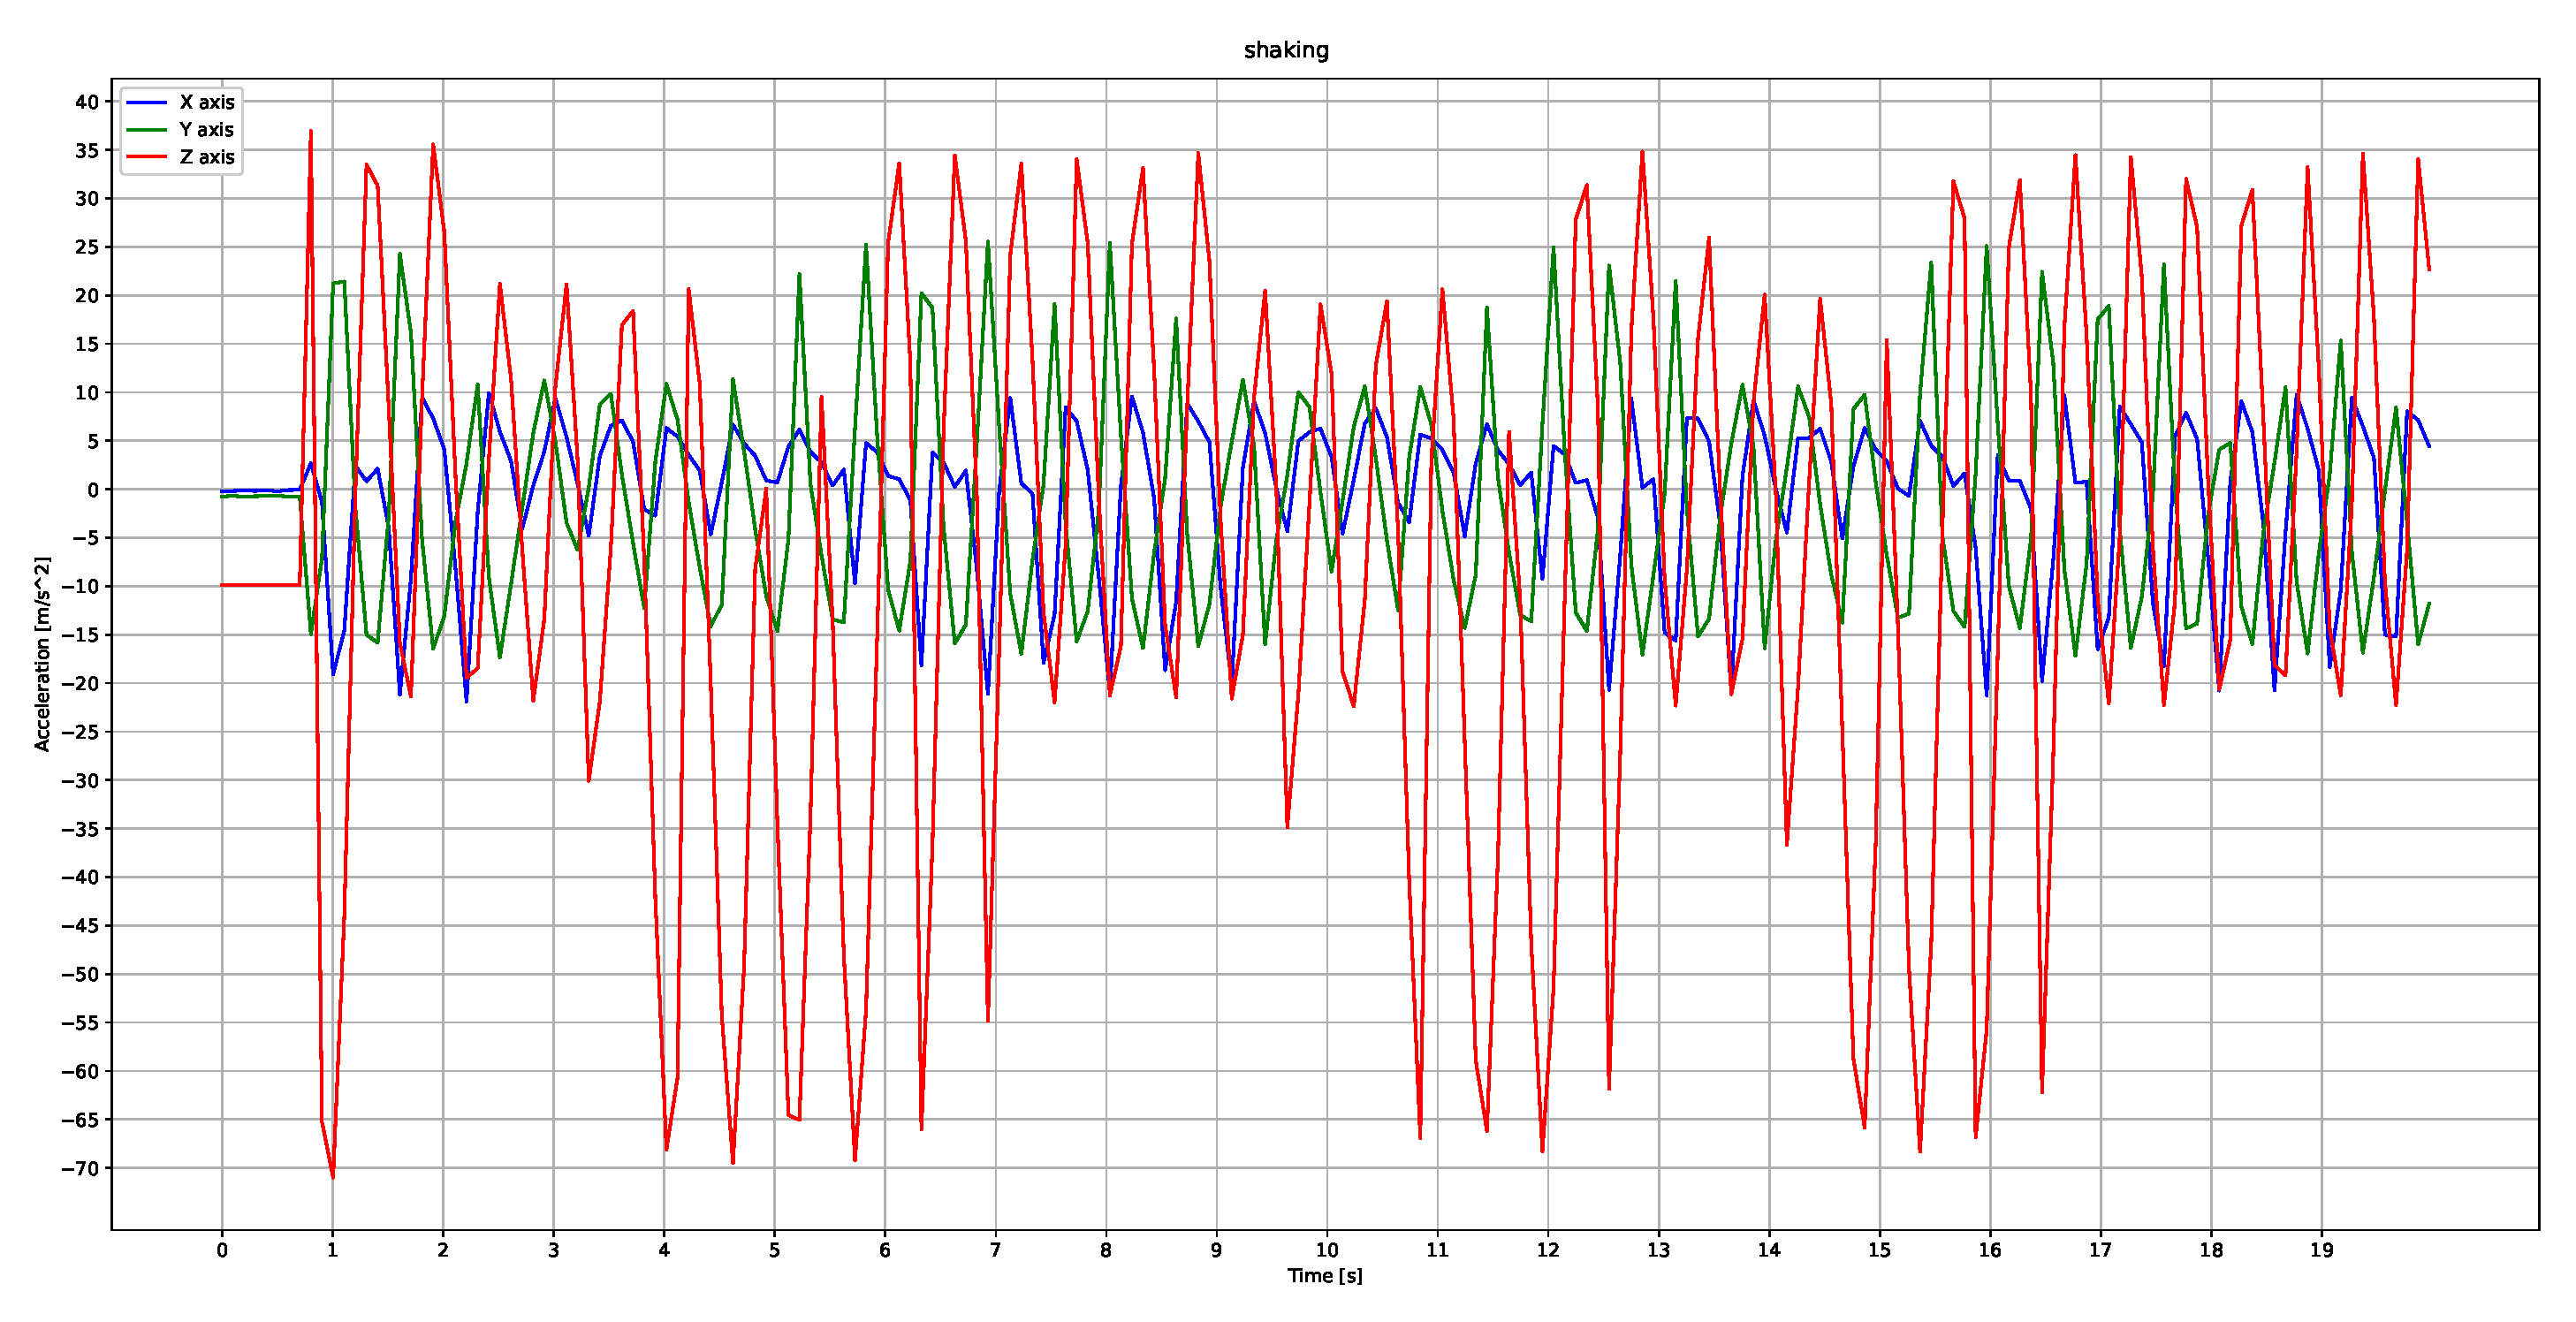
\includegraphics[width=0.8\textwidth]{resources/figures/Acceleration_shaking.eps}
    \caption{Accelerometer data during the shaking event}
    \label{fig:accelerometer_shaking}
\end{figure}

The Fourier analysis of the accelerometer data during the
shaking event is shown in
Figure \ref{fig:fourier_accelerometer_shaking}.
The Fourier analysis allows us to examine the
frequency components present in the accelerometer readings and
provides insights into the characteristics of the shaking motion.
By analyzing the frequency distribution and
identifying prominent peaks or patterns in the frequency domain,
we can gain a deeper understanding of the
dynamic response of the MediColbox to the shaking forces.


\begin{figure}[htbp]
    \centering
    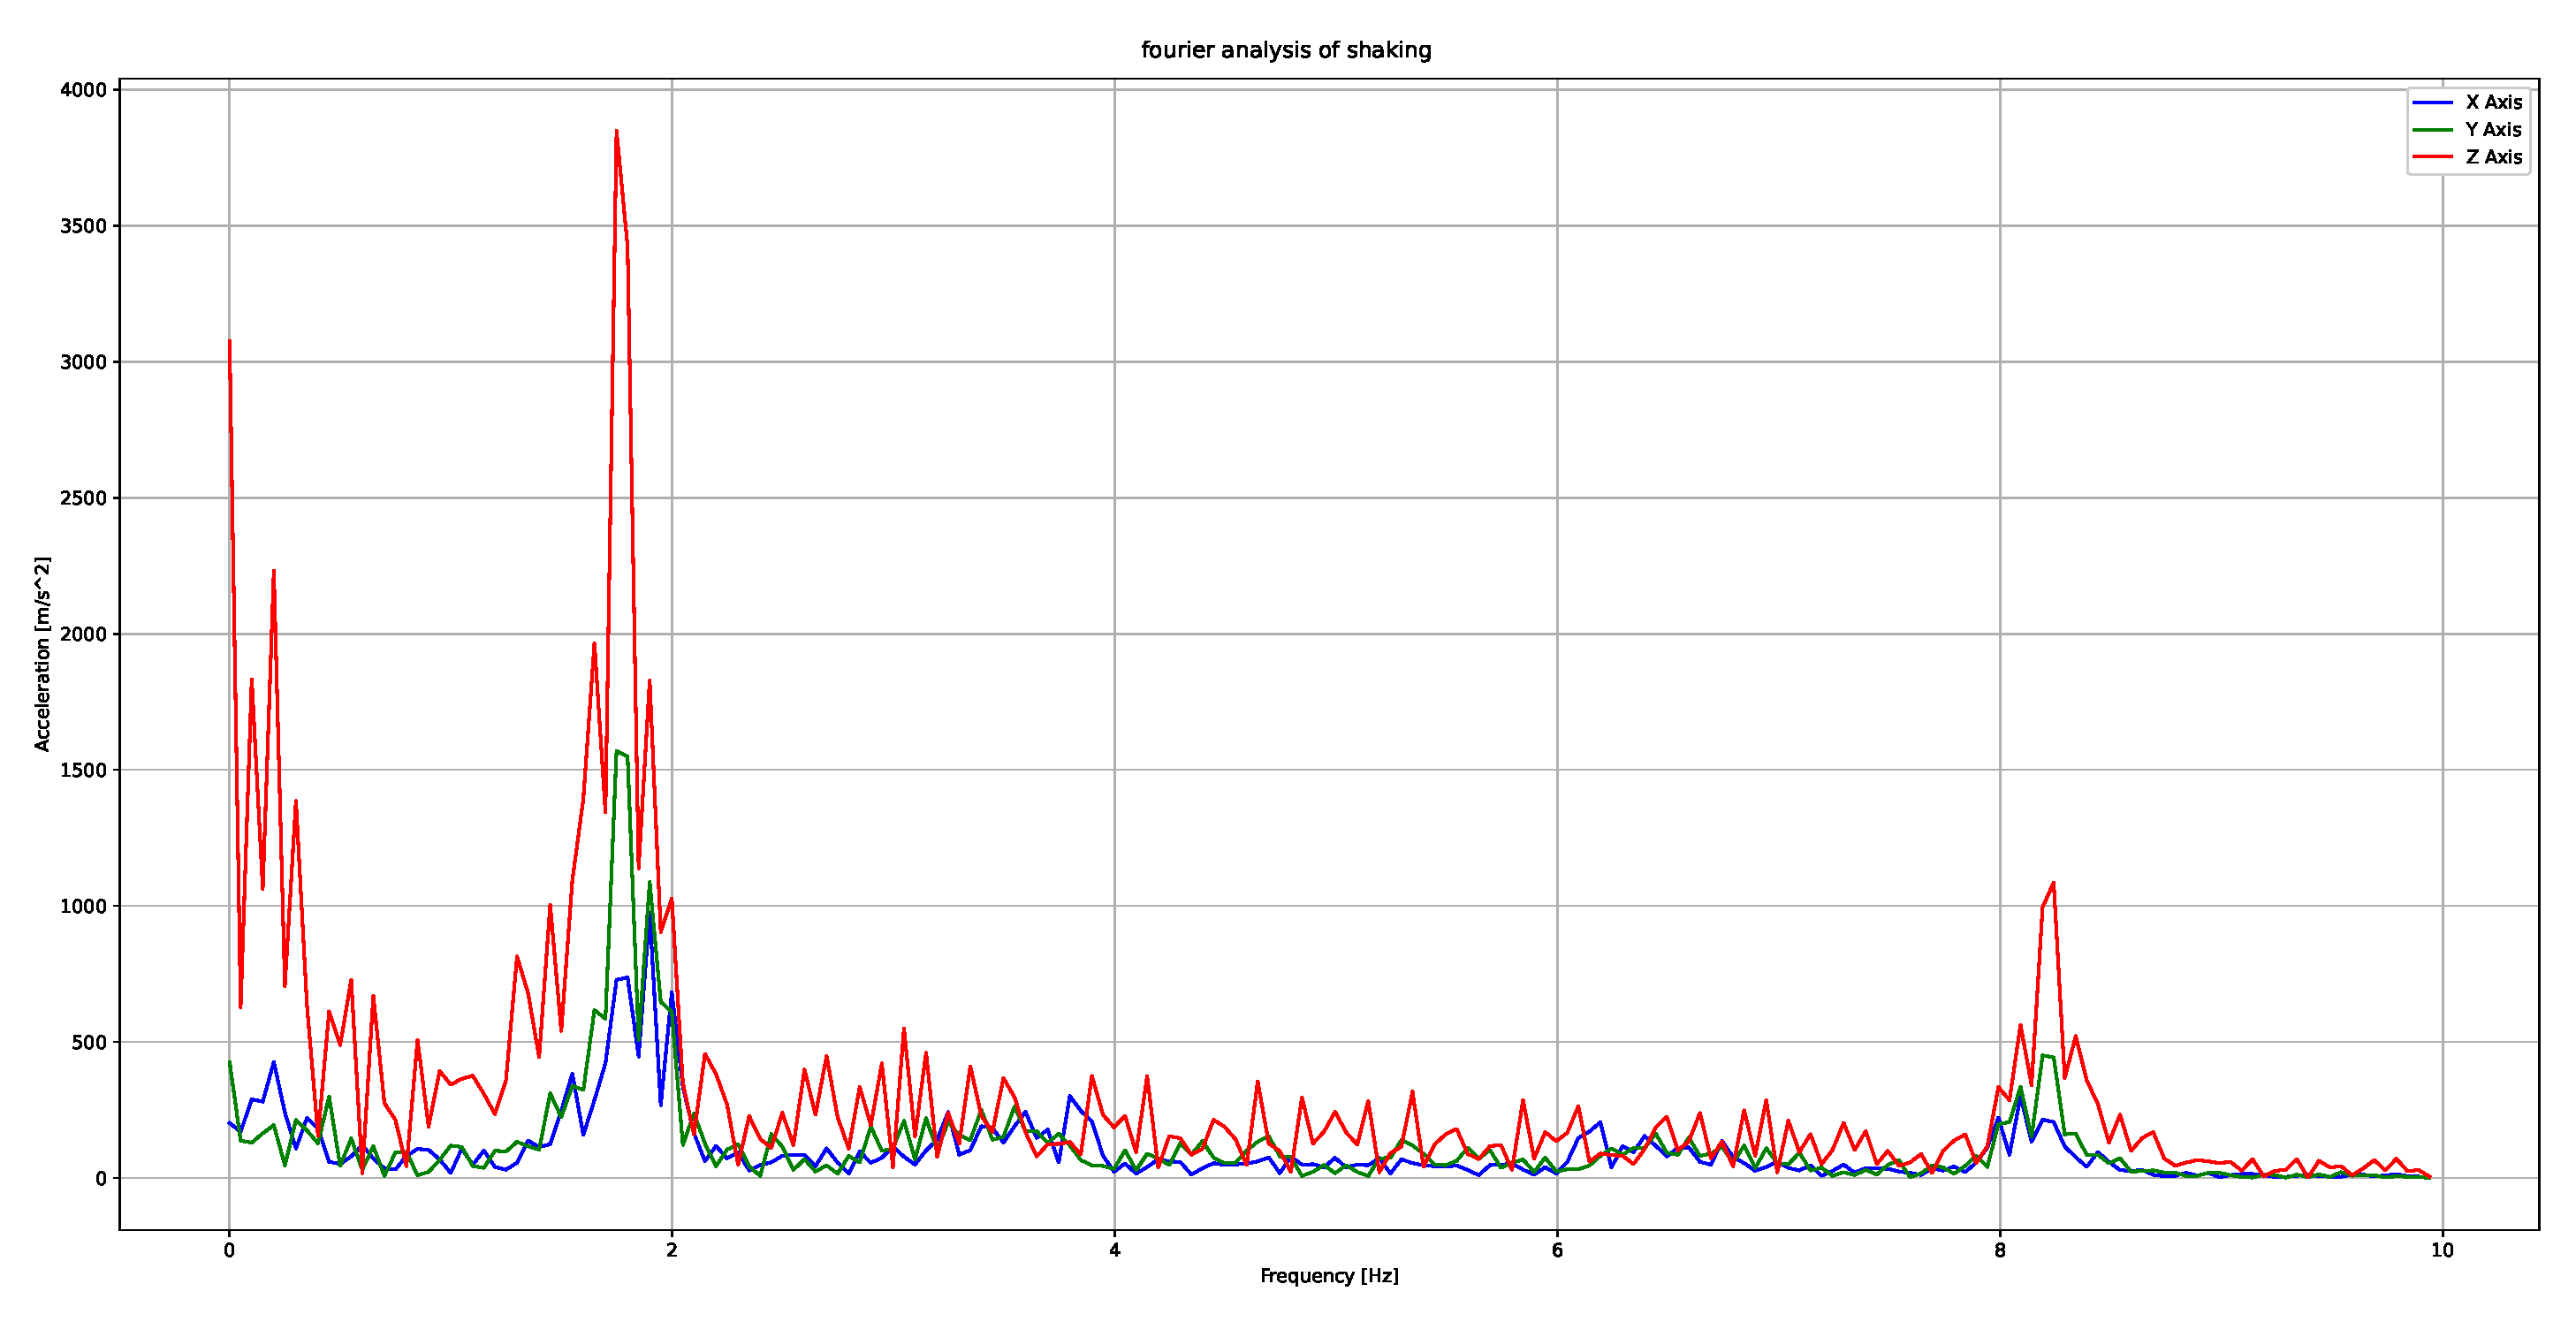
\includegraphics[width=0.8\textwidth]{resources/figures/Fourier_acceleration_shaking.eps}
    \caption{Fourier analysis of accelerometer data during the shaking event}
    \label{fig:fourier_accelerometer_shaking}
\end{figure}

\subsection{Discussion of Findings}

The analysis of the accelerometer data during the
simulated intrusion attempts provides valuable insights into the
IMU's ability to detect and capture unauthorized access events.
The results demonstrate that the
accelerometer readings accurately captured the
accelerative patterns associated with striking,
dropping, sawing, and shaking the MediColbox.

The findings suggest that the IMU is a reliable and
effective sensor for detecting physical movements and vibrations,
which are indicative of intrusion attempts.
The accelerometer data recorded during the
simulated scenarios showcased the IMU's sensitivity to
changes in acceleration,
enabling it to capture both high-impact events and
subtle vibrations.

However, it is important to note that the analysis
focused solely on the accelerometer data,
and other data collected by the IMU,
such as gyroscope or magnetometer readings,
were not considered in this study.
Further research could explore the
integration of multiple sensor data to enhance the
accuracy and robustness of intrusion detection.

Overall, the results indicate the potential of the IMU as
a standalone solution for intrusion detection on the
MediColbox. The findings support the feasibility of
utilizing the IMU to enhance the security and protection of the
MediColbox by effectively detecting and alerting on
unauthorized access attempts.

\end{document}